\usepackage{pdfpages}
\question \textbf{MST - Approximation}

\begin{parts}
\part Construct a complete graph with at least 6 nodes that satisfies the triangle inequality and apply the MST- approximation algorithm to approximate the optimal solution of the TSP.


\begin{solution}
Here goes the solution
\end{solution}


\part Prove that the MST-approximation is a 2-approximation of the TSP.


\begin{solution}
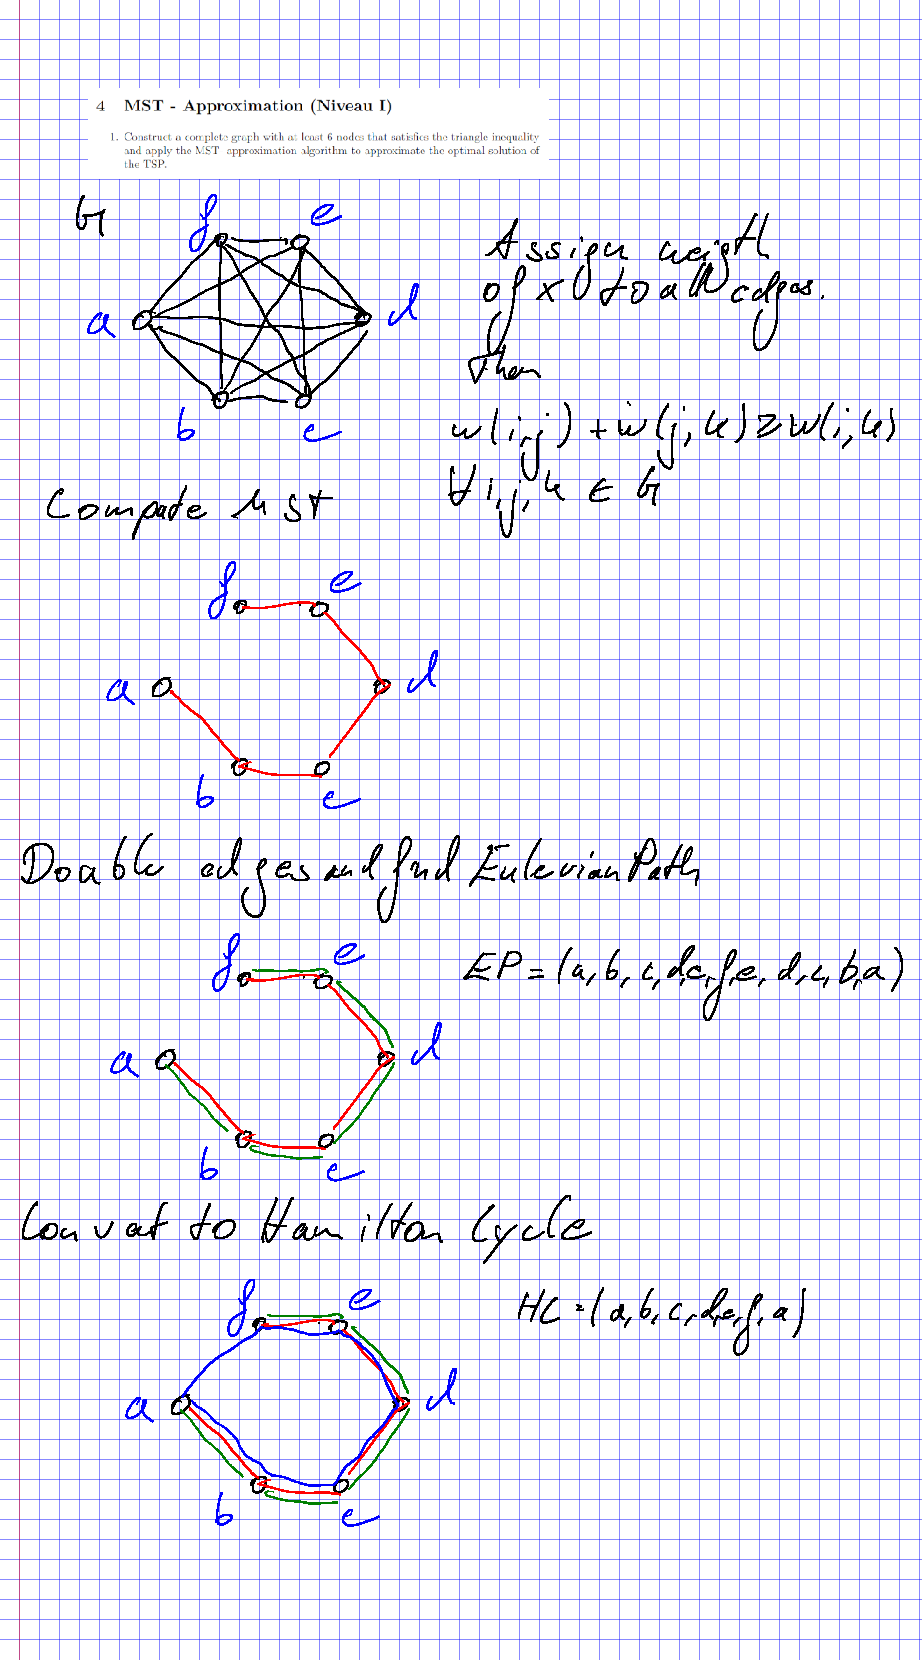
\includepdf[pages={1}]{task_4.pdf}
\end{solution}

\end{parts}


% For tasks without simply remove the \begin{parts}...\part...\end{parts} commands
